% Chapter Template

\chapter{Device fabrication and experimental methods} % Main chapter title

\label{Chapter5} 

\HRule
\vspace{0.5cm} \hspace{2cm}
\small
\hangindent=4cm
\\
        ``\emph{Scalability is the future}"
\\ \\
\hangindent=4cm
\begin{flushright}
--? \\
\end{flushright}

\vspace{0.5cm}

\noindent \HRule
\clearpage

\section{Device design} \label{sec:deviceDesign}

To propel the flip-flop qubit from theory to reality, we are using nanofabrication techniques to build the qubit, starting from a blank silicon wafer. We start with inventing designs for both the direct dipole-dipole coupling approach and coupling to a superconducting resonator that fulfil all requirements of the flip-flop qubit and comply with the fabrication tools available to us. 
From chapter \ref{Chapter2} we know what the flip-flop qubit requirements entail: We need to be able to readout the electron state, control the tunnel coupling, confine the electron at the interface and most importantly electrically control the donor both with DC voltages and fast pulses.
Additionally we would like an ESR antenna to be able to perform ESR and NMR on the electron and nuclear spin states separately from any flip-flop control, just like in a standard donor qubit device.  The following section describes how these requirements can be implemented for direct dipole-dipole coupling while section \ref{sec:designCPWR} discusses the resonator approach. 

\subsection{Flip-flop qubit} \label{sec:designFF}

\begin{figure}
	\centering
	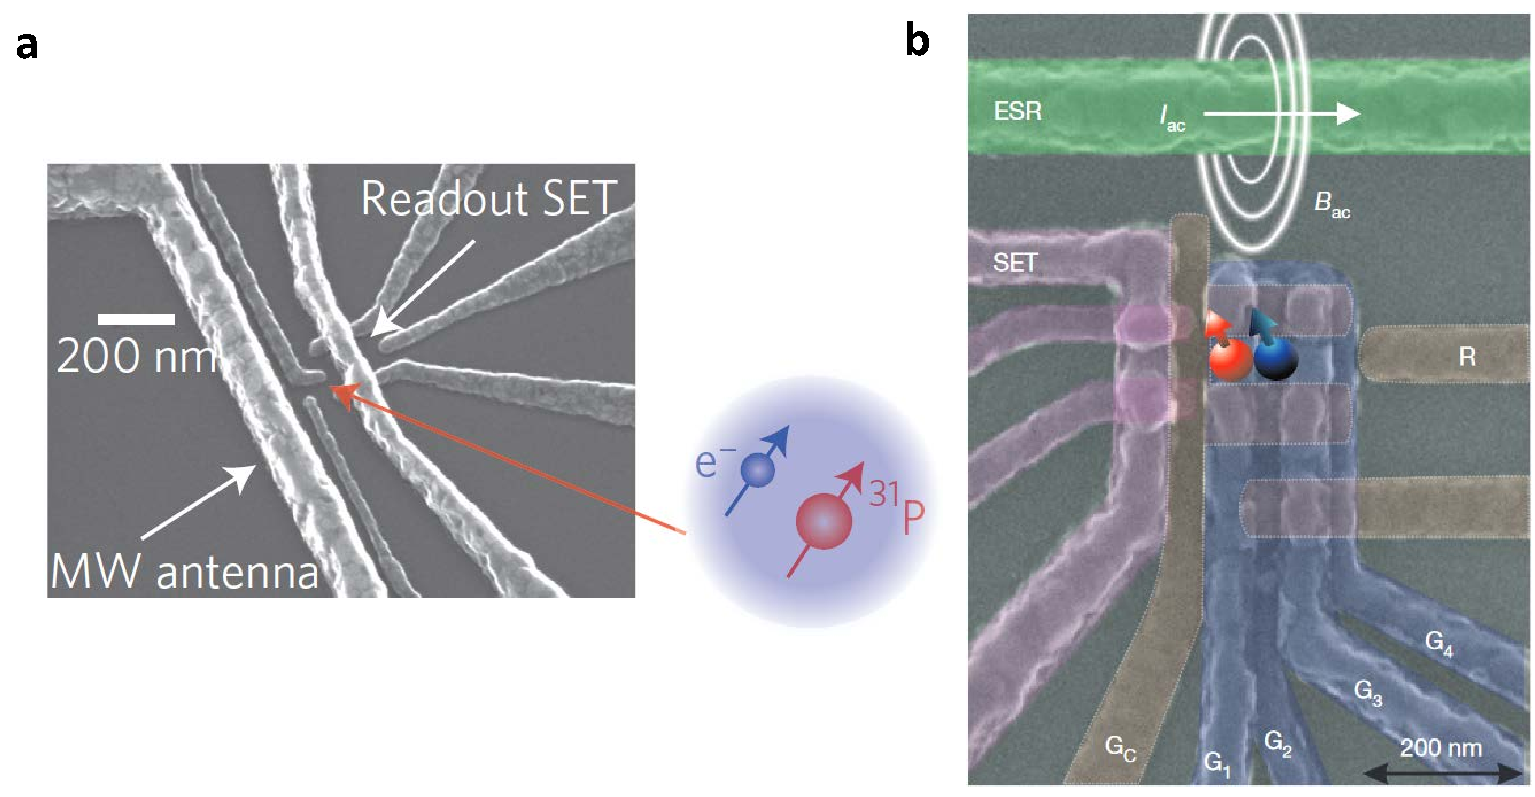
\includegraphics[width=0.8\textwidth]{polished/donorDot.pdf}
	\caption[Silicon donor and quantum dot qubit designs]{\textbf{Silicon donor and quantum dot qubit designs. a} Scanning micrograph of a typical phosphorus donor device in silicon. Both the electron and the nucleus can be operated as a qubit in this device structure \cite{Muhonen2014}. \textbf{b} Scanning micrograph of a typical CMOS quantum dot device in silicon which can be operated as a single or double quantum dot qubit \cite{Veldhorst2014}.}
	\label{fig:donorDotDevices}
\end{figure}

\begin{figure}
	\centering
	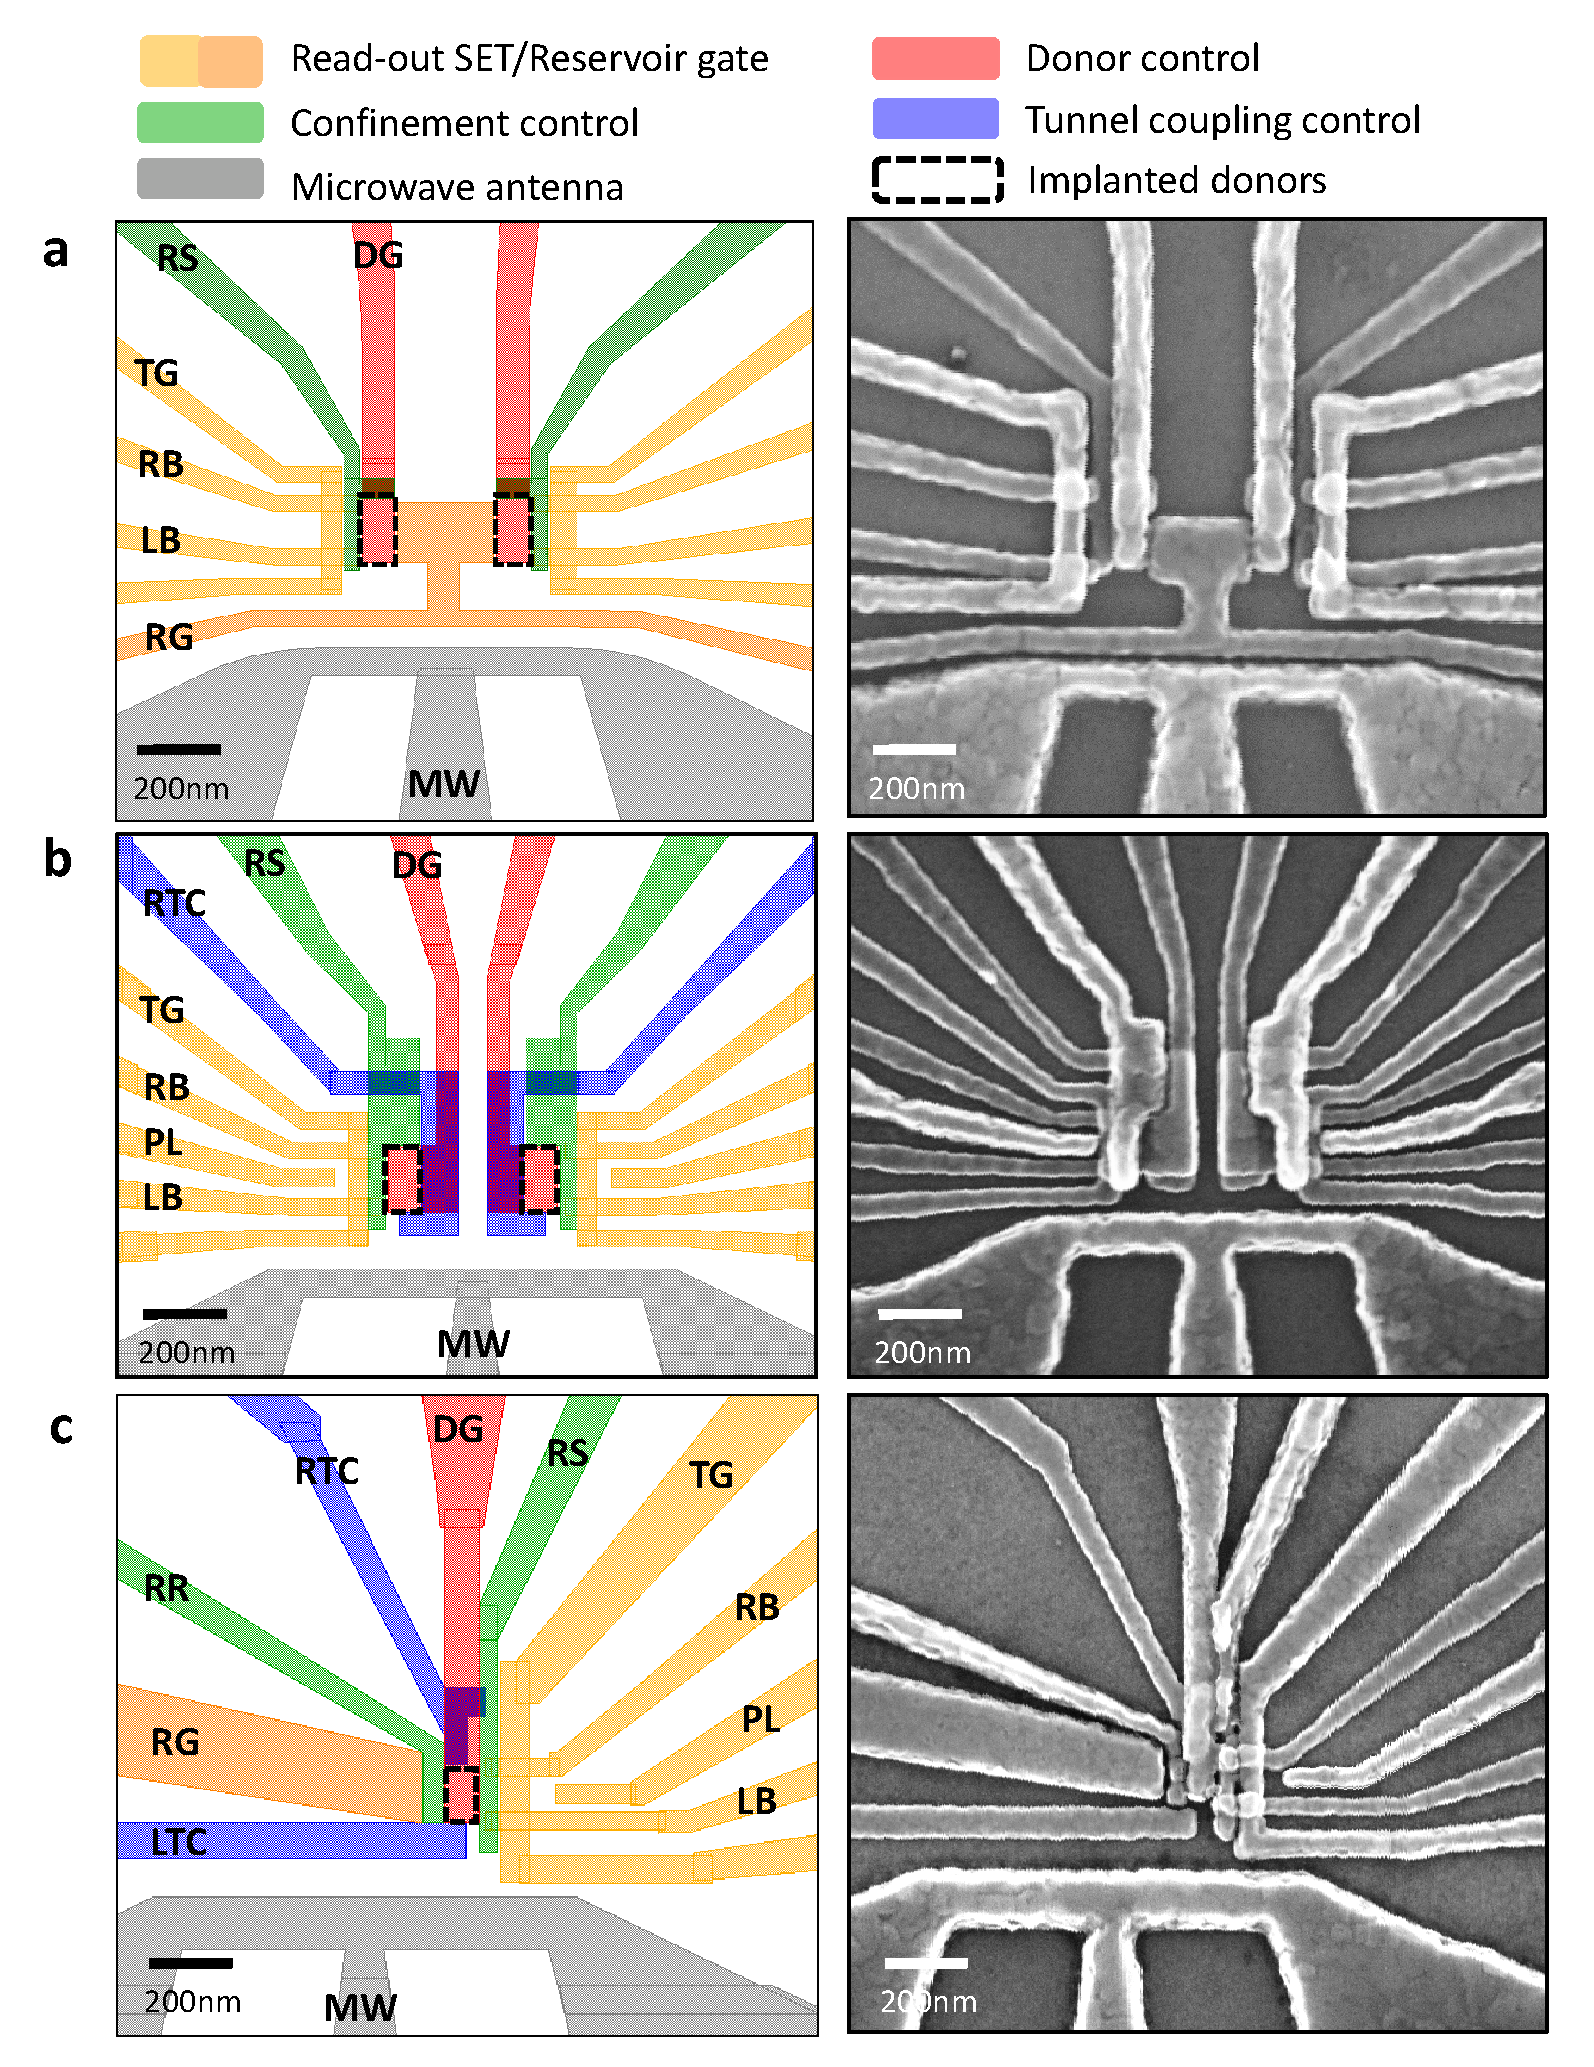
\includegraphics[width=\textwidth]{polished/FF_designs2.pdf}
	\caption[Flip-flop qubit designs for direct dipole-dipole coupling]{\textbf{Flip-flop qubit designs for direct dipole-dipole coupling. } The left column shows the flip-flop qubit design color-coded with gate purpose and gate labels while the right column shows the corresponding scanning micrograph of the finished devices. \textbf{a} Two-qubit flip-flop design with electron confinement control and reservoir for ease of readout. The confinement gate (RS, green) can also be used to modify the tunnel coupling within the voltage range set by the readout parameters. \textbf{b} Two-qubit flip-flop design with extended tunnel coupling control (RTC, blue). A plunger gate (PL, yellow) was added for increased adjustability of the SET. However the additional reservoir was removed. \textbf{c} Single flip-flop qubit device with full tunnel coupling control and readout adjustability.}
	\label{fig:designFF}
\end{figure}

We base our flip-flop qubit structure on existing donor and quantum dot structures (Fig.  \ref{fig:donorDotDevices}) that have made our research teams at UNSW very successful over the last decade \cite{Muhonen2014, Veldhorst2014}. We are working with donors in silicon but also separate the electron from the donor and confine it at the silicon interface - just like a quantum dot. Thus our flip-flop qubit will be a hybrid structure from the donor design shown in figure \ref{fig:donorDotDevices}a and the quantum dot design in figure \ref{fig:donorDotDevices}b. The first generation design of the flip-flop qubit is pictured in figure \ref{fig:designFF}a with a color-coded  layout on the left and an scanning micrograph image on the right. 

The key elements prominent in both donor and dot devices remain unchanged: We use a SET for electron readout (yellow), consisting out of two barriers ("right barrier" - RB, "left barrier" - LB) and a top gate (TG) with contact to a positively doped region ("source" - S and "drain" -D) (see section \ref{sec:qubit_initMeas}). Moreover we employ a coplanar microwave antenna (MW, grey) to supply microwave and radio frequency magnetic fields (see section \ref{sec:qubit_control}). 
We add a gate between the donor and the SET ("rate gate SET" - RS, green), like in the QD devices, to control the tunnel rate of the electron to the SET and prevent escape of the interface state. Additionally this gate can be used to tune the tunnel coupling. Most importantly we add an impedance matched gate on top of the donor to control the donor state and send fast electric pulses ("donor gate" - DG, red). 
However, we encounter one problem: To tune the tunnel coupling significantly we need to pull the electron horizontally by up to $100\,$nm. Consequently we choose an implantation window size of $60\times120\,$nm as indicated in figure \ref{fig:designFF}. Together with the necessary SET rate gate, this can lead to distances of the donor to the SET island of over $100\,$nm - too far for significant electron tunnelling for readout. To account for this difficulty we add an additional reservoir ("reservoir gate" - RG, orange, "reservoir source" - R). This brings two distinct advantages: Firstly, any donor close to either the SET island or the reservoir can be read out with the traditional donor readout (see section \ref{sec:qubit_initMeas}). Secondly, if the dot cannot be readout from the donor, we can readout the interface (quantum dot) state instead. Therefore we bias the donor such that the dot state becomes favourable, as shown in figure \ref{fig:ff_readout}. However, to avoid the electron from just escaping to the reservoir, we need to adjust the Fermi level of the reservoir such that the dot state lies below and will be occupied. During this process the SET Fermi level stays constant to provide charge sensing. 
We mirror this one-qubit structure at a distance of $200\,$nm to achieve a two-qubit device.

\begin{figure}
	\centering
	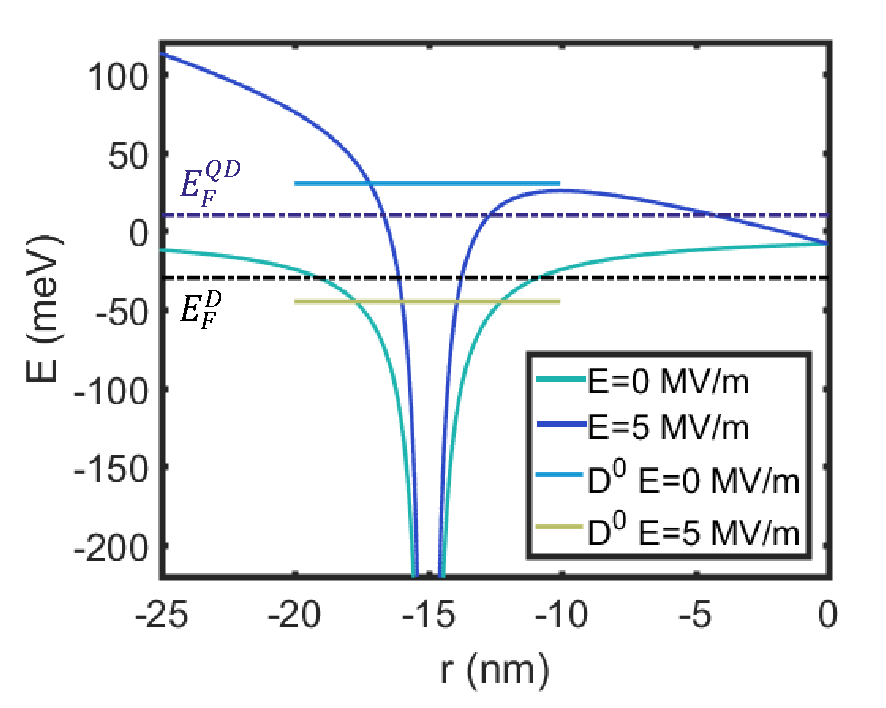
\includegraphics[width=0.8\textwidth]{polished/ff_readout.pdf}
	\caption[Flip-flop qubit readout energy diagram]{\textbf{Flip-flop qubit readout energy diagram. } Coulomb energy of the donor without and with an electric field of $5\,$MV/m applied. The $D_0$ donor ionization energy is $45.6\,$mV. At $r=0\,$nm the SiO$_2$ interface is positioned. The dotted lines show the reservoir Fermi level adjusted for an occupied donor (black) and dot state (blue). }
	\label{fig:ff_readout}
\end{figure}

In the following a few alternative, improved versions of this basic flip-flop structure are presented. Figure \ref{fig:designFF}b shows generation two where we added a plunger gate (PL, yellow) for better SET adjustment and an additional tunnel gate ("right tunnel coupling gate" - RTC, blue) to have higher control over the tunnel coupling, but at cost of the reservoir gate. 
Generation three (Fig. \ref{fig:designFF}c) incorporates both high tunnel coupling control with another tunnel coupling control gate added ("left tunnel coupling gate" - LTC, blue) and high adjustability for electron readout in form of an additional reservoir (RG), two rate gates ("rate gate reservoir" - RR and RS, green) and a plunger gate (PL). To achieve this highly controllable device however we had to sacrifice the second qubit. Thus this generation's focus will be one-qubit performance.
A few additional small design changes to be noted are: The SET rate gate as well as the plunger gate have been moved further away from the SET top gate to reduce the effect of strain on the 2DEG below the SET as this can prevent turn-on. Furthermore, the microwave short has been increased in both width and thickness to make it less susceptible to melting from sudden voltage fluctuations. 

\subsection{Coplanar waveguide resonator} \label{sec:designCPWR}

\subsubsection*{Simple resonator qubit design} \label{sec:simple_res_design}

\begin{figure}
	\centering
	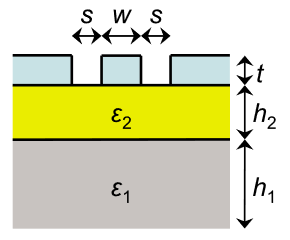
\includegraphics[width=0.4\textwidth]{polished/CPWR.png}
	\caption[Coplanar waveguide resonator geometry]{\textbf{Coplanar waveguide resonator geometry}. Geometric dimensions determining the impedance of a coplanar waveguide resonator.  }
	\label{fig:geometryCPWR}
\end{figure}

To couple our flip-flop qubit to a single photon we use a standard coplanar waveguide resonator (CPWR). This geometry consists out of a central conductor with a ground plane on either side. A cross section is shown in figure \ref{fig:geometryCPWR}. The waveguide width and gap size are chosen for an impedance of $50\,\Omega$ to $w=20\,\mu$m and $s=12\,\mu$m (factor $s/w=0.6$). The parameters are $\epsilon_{1}=11.6$, $h_1=500\,\mu$m for the silicon wafer, $\epsilon_2=3.78$, $h_2=8\,$nm for the silicon oxide layer and $t=50\,$nm for the superconducting film thickness  \cite{Jani2018}. 

We like to operate at a frequency $f_r\gg k_B T/h\approx 400\,$MHz to reduce thermal population, choosing $f_r\approx 6\,$GHz to keep component costs low.  We operate the fundamental mode of a $\lambda/2$ resonator which determines the resonator length to $l=c_0/2\sqrt{\epsilon_{\rm eff}\epsilon_0}\cdot f_r$. $\epsilon_{\rm eff}$ is the effective permittivity of the wave guide which can be estimated to $\epsilon_{\rm eff}=(1+\epsilon_1)/2=6.3$ \cite{PalaciosLaloy2010}. Figure \ref{fig:designCPWR}a shows the CPWR design. 

\begin{figure}
	\centering
	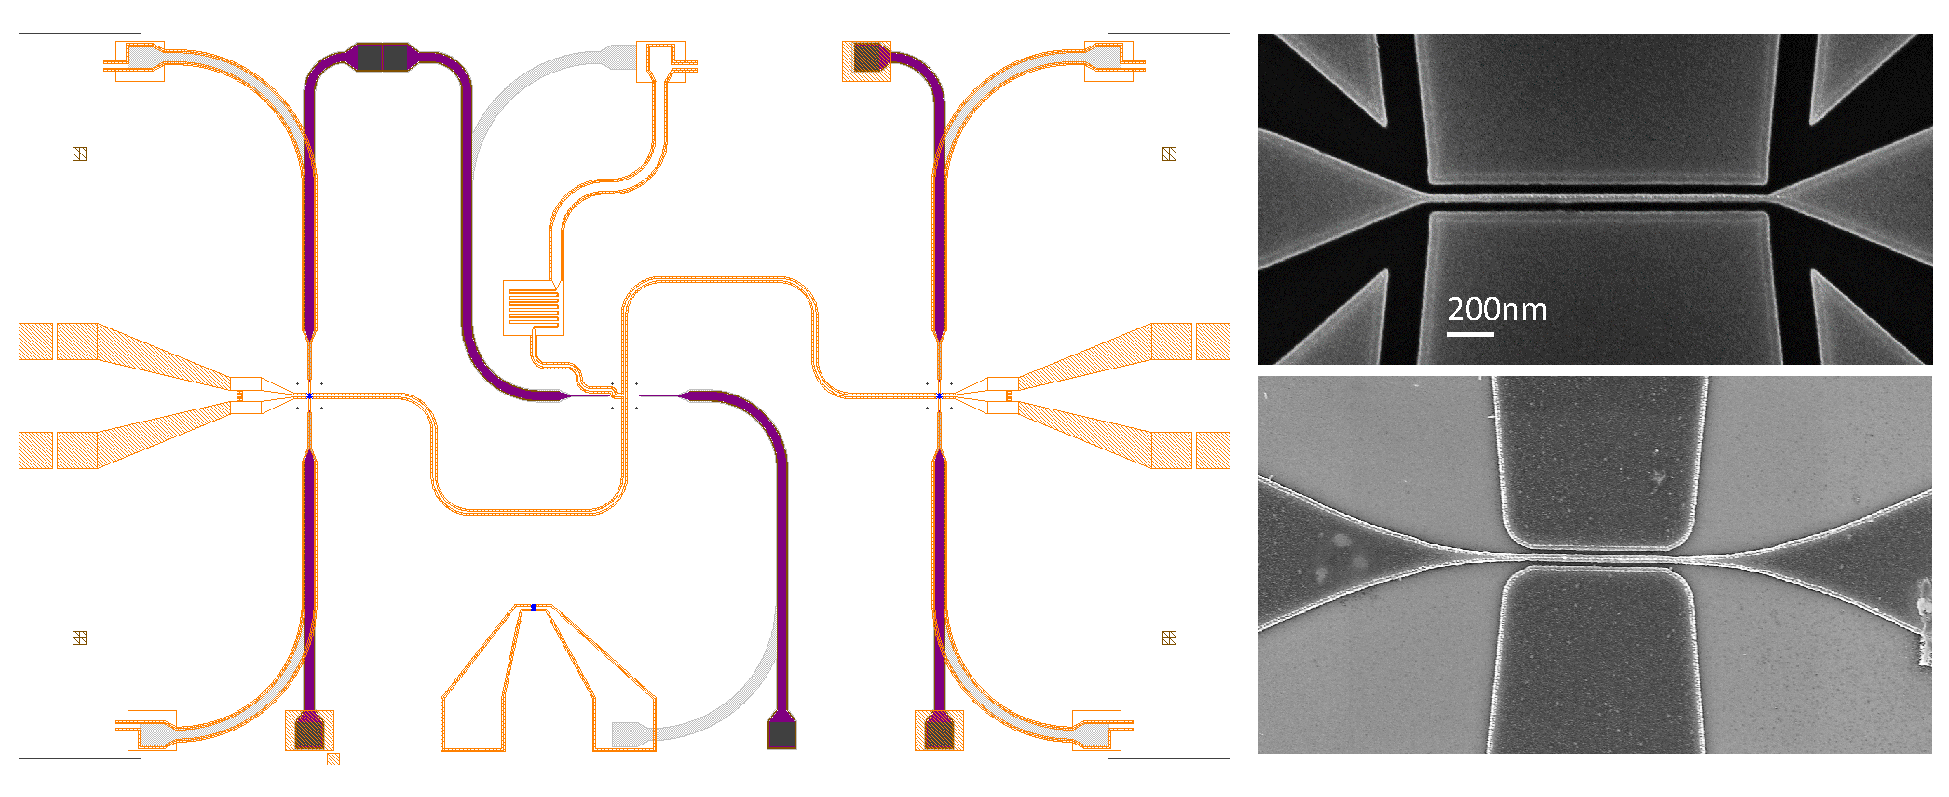
\includegraphics[width=\textwidth]{polished/CPWR_designs.pdf}
	\caption[Simple CPWR qubit design]{\textbf{Simple CPWR qubit design. a} Overview of the CPWR design, color-coded with feature purpose. The sample is covered in a superconducting film with etched regions indicated in orange and green. Purple shows the n+regions with their respective Ohmic contacts in black. The active qubit region, the capacitors and the inductor are shown zoomed-in in \textbf{b} to provide details. \textbf{b} Inductor and capacitor example designs and active qubit region with gate labels. \textbf{c} Scanning micrograph overview of the CPWR. \textbf{d, e} Scanning micrograph of the active qubit region for two different designs. }
	\label{fig:designCPWR}
\end{figure}

The coupling of the resonator to the lines is determined by the capacitor design at each end of the resonator, acting as a semi-reflecting mirror, introducing a strong impedance mismatch. We are aiming for the over-coupled regime where the coupling exceeds the internal losses. We simulate the capacitor size in the computer simulation theory (CST) microwave studio. Ultimately however, we rely on testing different designs as we are operating in the single photon regime where the coupling strength is mainly determined by quantum tunnelling. Figure \ref{fig:designCPWR}b shows an example capacitor design. As we are working in transmission mode we place one capacitor at each end of the resonator. 

Now we integrate our spin qubit into the resonator design by placing several phosphorus donors directly beneath the resonator central conductor (CC). However, we require a vacuum electric field amplitude of $E_{\rm vac}\approx 30\,$V/m to achieve high qubit-resonator coupling rates (see chapter \ref{sec:cqed_ff}, \cite{Tosi2017}). These electric field amplitudes can be reached by narrowing the central conductor in the active qubit region to around $100\,$nm as shown in figure \ref{fig:designCPWR}b \cite{Samkharadze2016}. In order to load electrons to the donors, we incorporate two reservoir gates ("top top gate" - TT and "bottome top gate" - TB) with respective n+ regions and Ohmic contacts ("source" - S and "drain" - D) for each active region which have the ability to bring a 2DEG close to the qubit.

 Finally, we need to apply a bias to the qubit to move the electron. Thus we have to bias the center conductor. Therefore we add a DC feed line at the electric field node at the center of the resonator. High frequency noise is filtered with an on-chip inductor as shown in figure \ref{fig:designCPWR}a,b. 
 
Figure \ref{fig:designCPWR}c-e shows scanning micrographs of the fabricated resonator devices. 

Due to the large metallic ground plans involved in this design, electrostatic discharge (ESD) can be a serious problem with charges accumulating on the metal during fabrication and chip handling. Consequently we removed tips channelling voltage as in figure \ref{fig:designCPWR}d (improved design in figure \ref{fig:designCPWR}e) and grounded all gates to the large ground planes by leaving small strips of metal unetched. After a device has been mounted to an enclosure (see section \ref{sec:packaging}) and all gates are grounded, these strips can be disconnected by scratching with a diamond-tip pen or scriber. 

\subsubsection*{Advanced resonator qubit design} \label{sec:adv_res_design}

While the design presented in the previous section is proficient to operate a flip-flop qubit in its most basic functionality with a bit of luck in the donor position and depth (see chapter \ref{sec:res_chargequbit}), its qubit control capability is very limited. The reservoir gates allow biasing, however they are far away from the qubit due to fabrication limitations (see chapter \ref{sec:fab_cpwr}) and thus wave function control will be very limited if not impossible. Furthermore, many electrons can be loaded under the central conductor during qubit loading. 
To mitigate these issues we are developing a design both more robust against implantation uncertainties as well as allowing higher qubit control. Figure  \ref{fig:designCPWR_new}) shows the current advanced design.  

\begin{figure}
	\centering
	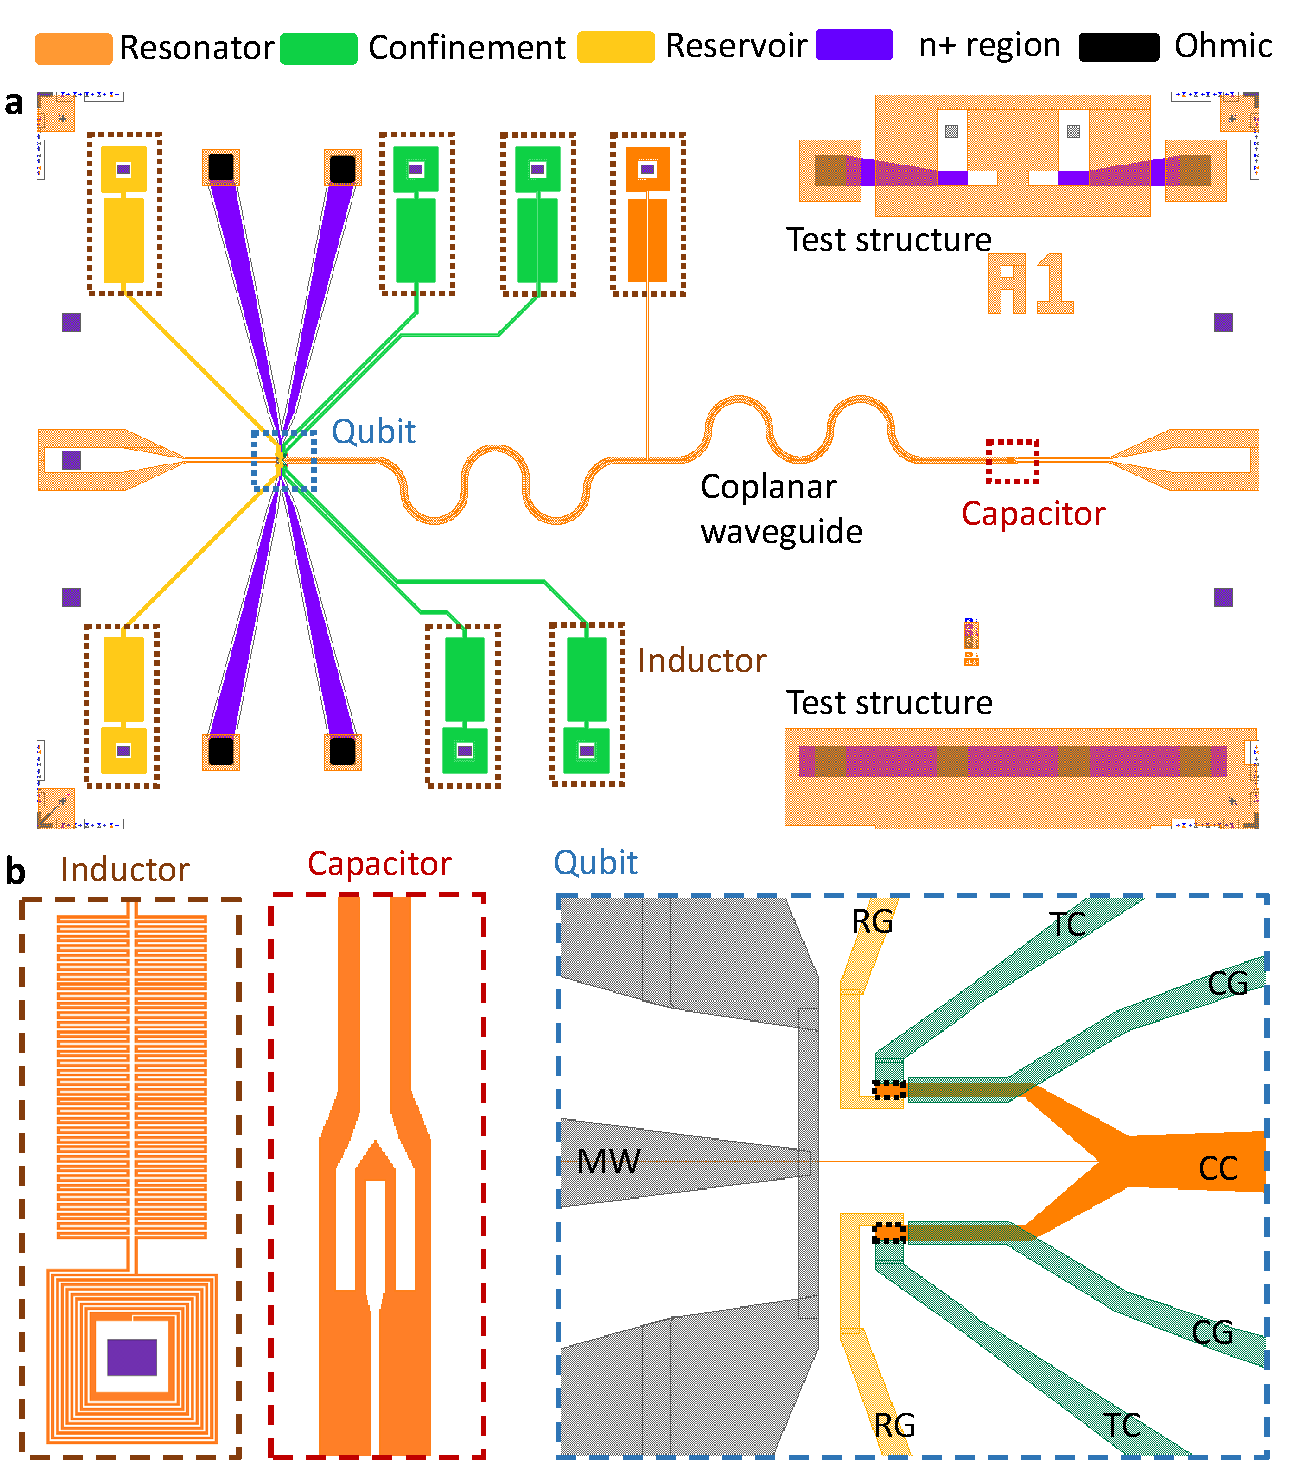
\includegraphics[width=0.9\textwidth]{polished/CPWR_VS.pdf}
	\caption[Advanced CPWR qubit design]{\textbf{Advanced CPWR qubit design. a} Overview of an advanced resonator flip-flop qubit structure, color-codes with feature purpose, which includes several control gates and is operated in reflection. \textbf{b} Detailed view of example inductor and capacitor as well as the active qubit region with gate labels.   }
	\label{fig:designCPWR_new}
\end{figure}

The main difference between the advanced and the simple design is that now we use a two-layer Aluminium structure in the active qubit region (Fig. \ref{fig:designCPWR_new}c), allowing for a much smaller feature size and a more complex gate layout. Furthermore we now operate the resonator in reflection. We have only one active region but fit two qubits inside it. Both have a separate reservoir ("reservoir gate" - RG, yellow) as well as two gates to confine the electron and control tunnel coupling ("tunnel coupling gate" - TC and "confinement gate" - CG, green). Each of these gates has its own on-chip inductor to allow for loss-less DC biasing. We also incorporate a microwave antenna into our design to allow for individual electron and nuclear spin control. 

\section{Device fabrication} \label{sec:fabrication}

\subsection{Silicon wafer} \label{sec:fabWafer}

\begin{figure}
	\centering
	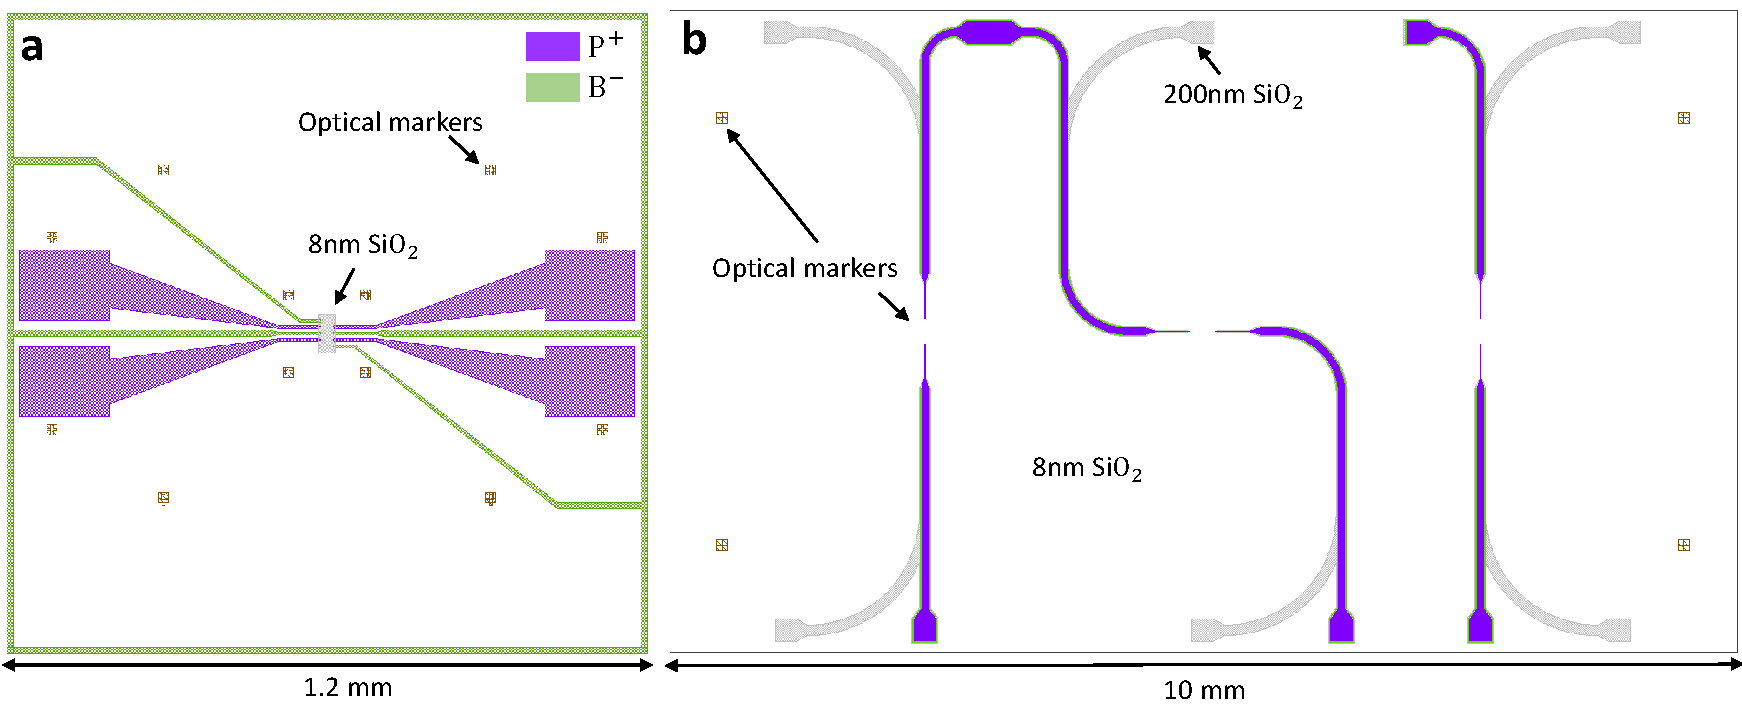
\includegraphics[width=\textwidth]{polished/stock.pdf}
	\caption[Silicon wafer layout]{\textbf{Silicon wafer layout.} Layout of the features patterned on the silicon wafer during wafer preparation for the standard Aluminium devices (\textbf{a}) and the resonator devices (\textbf{b}). 
	%n+ and p+ regions are created with phosphorus and boron diffusion respectively (purple, green). A thin and a thick silicon oxide is grown and optical markers are etched and evaporated
	 }
	\label{fig:wafer}
\end{figure}

All devices start off as a bare silicon wafer. For testing, natural silicon wafers with low residual p-type background doping ($\sim 10^{12}\,\rm{cm}^{-3}$) are used, while highly precise qubit experiments are performed on wafers with an $800\,$nm epitaxial layer of isotopically purified $^{28}$Si on top of $500\,\mu$m thick high purity natural silicon, provided by K. Itoh. The $^{28}$Si has a residual concentration of $730\,$ppm of $^{29}$Si and $30\,$ppm $^{30}$Si.

The first step after acquiring a new wafer is a thorough clean. Then optical alignment marks are etched into the silicon. Next the wafers are doped firstly with Boron ($B^-$) to create positively charged guard rings. These guards prevent leakage at the Si-SiO$_2$ interface when positive charges trapped in the wet field oxide induce an unintentional two-dimensional electron gas (2DEG). Then phosphorus ($P^+$) is diffused to create $n+$ regions to form the source and drain contacts. Afterwards $200\,$nm of field oxide are grown in a wet thermal oxidation furnace. Next, the field oxide is removed in the active qubit region to be replaced by a $8\,$nm ($2\,$nm for CPWR style devices) of high quality gate oxide, grown in an ultra-dry furnace. Lastly micrometer sized markers formed out of Platinum on top of Titanium (TiPt markers) are patterned for course alignment with electron beam lithography (EBL). Figure \ref{fig:wafer}a shows an the design of a standard qubit wafer after this initial processing. 

The processing of wafers designated for coupling to superconducting resonators is done in the same way. The only noticeable difference is that most of the wafer is the active region and thus only where the top gates are indented, a thick field oxide is grown. This wafer design is shown in figure \ref{fig:wafer}b. 


\subsection{Nano-fabrication process - standard aluminium devices} \label{sec:nanofab_al}

Once the silicon wafers have been prepared, they are diced into smaller chips for different projects. While all silicon donor aluminium style devices use inherently a very similar fabrication process, small differences occur due to individual preferences and cleanroom superstition. In the following the process specific to the flip-flop qubit used by the author in this thesis is presented. 

\paragraph*{Cleaning}
To remove any residue of resist or other contaminants the chips are cleaned by soaking them first in acetone and subsequently in Isopropyl alcohol (IPA) for each 10 min while applying ultrasound. The cleaning process is finished with 10 min of oxygen plasma ashing. 

\begin{figure}
	\centering
	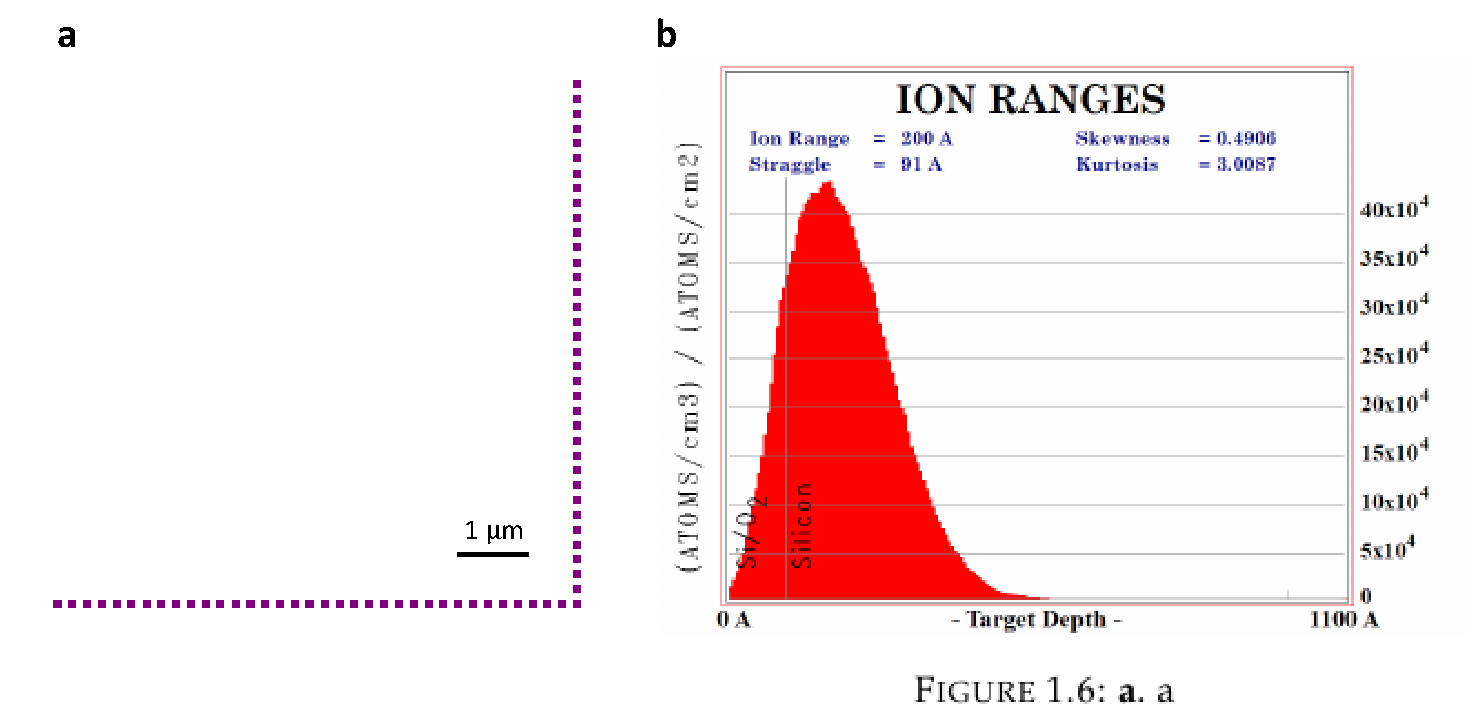
\includegraphics[width=0.9\textwidth]{polished/implantion_TiPtmarks.pdf}
	\caption[TiPt marker design and ion distribution for implantation]{\textbf{TiPt marker design and ion distribution for implantation a.} Design of the nanometric TiPt markers used for EBL alignment of the different layers. The individual square design is robust against melting during RTA. \textbf{b} Distribution of ions with depth for an acceleration voltage of 12keV of P$^+$ ions with a fluence of $2\cdot10^{11}$/cm$^2$.   }
	\label{fig:TiPtmarks_impl}
\end{figure}

\paragraph*{TiPt markers}
The first processing step is the formation of the nanometric markers in each pixel which enable alignment of different layers during EBL. These markers need to withstand temperatures of $1000\,\degree$C during subsequent processing steps. Therefore we use Platinum which not only has a very high melting point of $1763\,\degree$C but also has a high atomic number resulting in good contrast on the electron beam microscope. For adhesion to the silicon oxide surface we add a thin layer of Titanium with a melting point of $1668\,\degree$C. Regardless of these high melting points, large TiPt structures melt and deform. Consequently we use marker shapes consisting out of many small $100\times100\,$nm squares as shown in figure \ref{fig:TiPtmarks_impl}a which survive our high temperature process. 
We create these markers using EBL.

\textit{Standard EBL process:} We first bake our chip at $180\,\degree$C for 10 min and then spin polymethyl methacrylate (PMMA) A4 resist with $4000\,$rpm for 40s with 10s of $8000\,$rpm finish. This gives a resist thickness of $200\,$nm. The resist is then baked for 90s at $180\,\degree$C. Droplets of colloidal gold solution can be placed on the corners of the chip as focus markers. The pattern is written with a RAITH150-Two EBL system with an acceleration voltage of $30\,$keV and a dose of around $500\mu C/cm^2$, depending on aperture, feature size and geometry. After exposure, the resist is developed for 40s in a 1:3 solution of methyl-sobutyl-ketone (MIBK) and IPA and for 20s in IPA with a 5s ultrasound finish. 
Subsequently 15nm of Titanium and 65nm of Platinum are evaporated by electron beam physical vapour deposition (EBPVD). Then the chip is placed in N-methyl-2-pyrollidone (NMP) at $80\,\degree$C for 5min to perform lift off. 

\paragraph*{Donor implantation}
The next step is the implantation of our phosphorus donors. Therefore a PMMA mask of dimensions  $120\times60\,$nm is patterned with EBL in each pixel ("implantation window"). We require a donor depth of around 10-15nm below the silicon oxide. As the tunnel coupling between the donor and dot can be reduced but not increased we aim for 10nm. An acceleration voltage of 12keV of $P^+$ ions complies with this requirement as the simulated ion depth distribution in figure \ref{fig:TiPtmarks_impl}b shows. We'd like 8-10 donors in our implantation window which corresponds to a fluence of $2\cdot 10^{11}/cm^2$ and an average donor distance of 25nm. The implantation is performed by Jeff McCallum. After the implantation is completed the resist is removed and the chip undergoes rapid thermal annealing (RTA) for 5s at $1000\,\degree$C. This activates the donors and repairs the damage caused in the silicon lattice by the ion implantation \cite{McCamey2005}. 

\paragraph*{Ohmic contacts}
Finally Aluminium Ohmic contacts to the diffused $n+$ regions are formed and activated with a forming gas anneal (FGA) (N$_2\ 95\%$, H$_2\ 5\%$) at $400\degree$C for 15min in the clean anneal furnace and the chip is diced into 4x4 pixel pieces for individual processing. 

\paragraph*{Multi-layer Aluminum nanostructures}

\begin{figure}
	\centering
	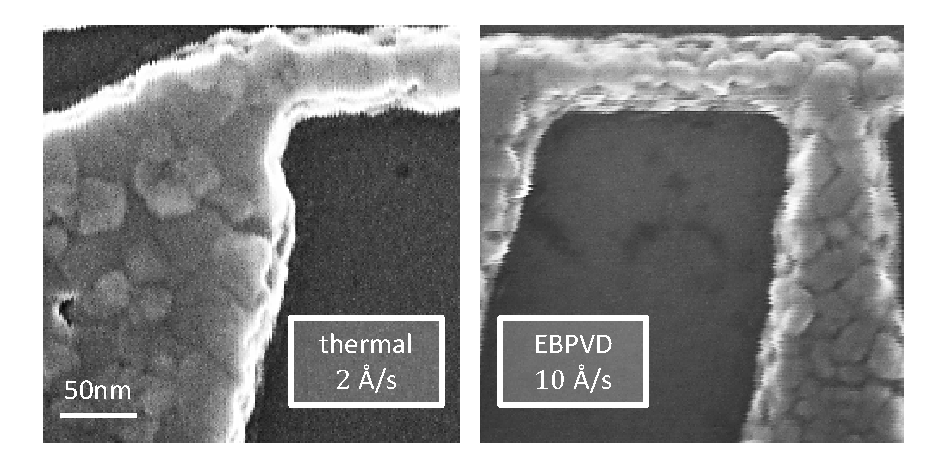
\includegraphics[width=0.7\textwidth]{polished/grainsize.pdf}
	\caption[Aluminium grain size for thermal evaporation and EBPVD]{\textbf{Aluminium grain size for thermal evaporation and EBPVD. a} Aluminium structure evaporated at a rate of $2\,\Angstrom$/s in a thermal evaporator. The grains are 30-50nm large. \textbf{b} Aluminium structure evaporated at a rate of $10\,\AA$/s with EBPVD. The grains are 10-30nm large. }
	\label{fig:grainsize}
\end{figure}

On each 4x4 pixel piece three layers of aluminium gates on top and around the implantation window are added. For each layer the piece undergoes the following steps. 
First the piece is cleaned, then PMMA resist is spun and exposed during EBL as described above for the TiPt markers. After development aluminium is evaporated either in a thermal or an EBPVD evaporator. Tests have been performed and we find that the evaporation rate and its stability directly influences the aluminium grain size. Thermal evaporation can be unstable due to a fluctuating current and is restricted to rates below $3\,$\AA/s. Thus it regularly leads to a larger grains than EBPVD where evaporation rates of $10\,$\AA/s can be achieved - see figure \ref{fig:grainsize}. With EBPVD we evaporate 25nm, 45nm and 80nm subsequently for the different layers and lift off in hot NMP for 1.5-3h. During the following oxygen plasma ash and baking, the outer $2-3\,$nm of each aluminium layer are oxidized to form an electrically insulating layer. Figure \ref{fig:ff_layers} shows the layer schematic and each layer individually. 

\begin{figure}
	\centering
	\includegraphics[width=\textwidth]{polished/FF_layers.pdf}
	\caption[Aluminium layer arrangement of the dipole flip-flop qubit]{\textbf{Aluminium layer arrangement of the dipole flip-flop qubit.} Qubit gate layout color-coded for the three layers and corresponding scanning micrograph images for each layer.}
	\label{fig:ff_layers}
\end{figure}

\paragraph*{Finish}
After the last layer has been completed, the piece is cleaned one more time and FGA is performed to passivate any charge traps at the Si-SiO$_2$ interface\cite{Brower1988}.

\subsection{Nano-fabrication process - resonator devices} \label{sec:fab_cpwr}

As our research group had not fabricated any form of superconducting devices before, we started building up a new process which is still undergoing development. This section describes the fabrication performed for the measurements presented in this thesis and gives an outlook for new, more sophisticated resonator devices. 

\begin{figure}
	\centering
	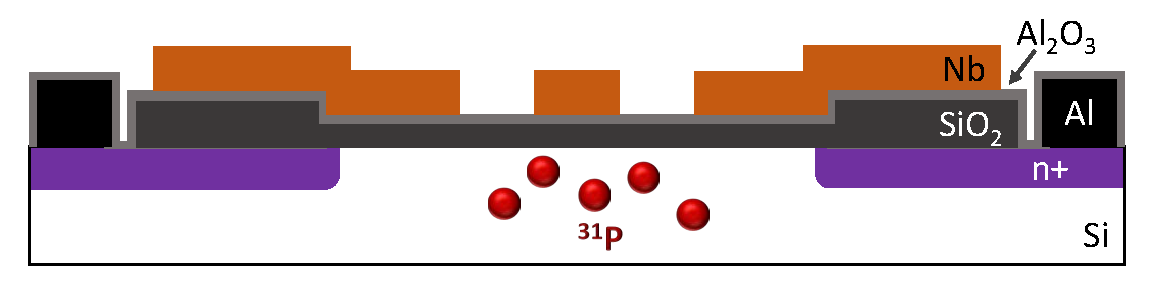
\includegraphics[width=0.9\textwidth]{polished/fab_cpwr.pdf}
	\caption[SEM FF]{\textbf{a}. a }
	\label{fig:fab_cpwr}
\end{figure}

\paragraph*{Cleaning} 
First the wafer is cleaned in the same way as for the aluminium devices. However, once the niobium layer has been deposited, oxygen ashing oxidises the niobium to a degree that compromises the quality of the superconducting film, thus will not be performed.

\paragraph*{Donor implantation}
The next step is the implantation of our phosphorus donors. Therefore a photo mask of dimensions  $44\times24\,\mu$m is patterned with photo-lithography in each pixel (implantation window). We implant $P^+$ ions with an acceleration voltage of 11keV and a fluence of $1\cdot 10^{11}/cm^2$ which corresponds to an average donor distance of 38nm. The implantation is performed by Jeff McCallum. After the implantation is completed the resist is removed and the wafer undergoes RTA. Finally Aluminium Ohmic contacts to the diffused $n+$ regions are formed and activated with a FGA.

\paragraph*{Sputtering}
First we apply a thin layer of Al$_2$O$_3$ to serve as an etch stopper. With atomic layer deposition (ALD) we run 30 cycles at $250\,\degree$C which gives 3 nm. 
Then the wafer is sent to CSIRO at Lindfield where the 50nm of niobium are sputtered. However, the film thickness fluctuates between $30-40\,$nm which is determined with a stylus profilometre. Using a 4-point measurement we find these films to have a resistance of $15\,\Omega$ at room temperature. 

\paragraph*{Resonator structures}
To pattern our resonator structures we spin PMMA resist and expose it with EBL. In contrast to the aluminium style devices, we write what will be removed. Moreover, the resonators are larger than one write field. To create a smooth coplanar waveguide we employ the fixed beam moving stage (FBMS) technique that moves the stage below the beam for the entirety of the device, thus apprehending stitching issues. After patterning we develop the sample. Then we perform hollow cathode reactive ion etching (HC RIE) with a gas mixture of 20sccm CF$_4$ and 10sccm Ar at a pressure of 5Pa with 50W power to remove the Nb not protected by our PMMA mask. This process needs to be carefully calibrated so that after the etch duration the Nb is fully removed but the PMMA mask is still protecting the remaining Nb surface. For this purpose we always add test samples to the process. After etching the sample is cleaned and ready for packaging. 

\paragraph*{Outlook for advanced resonator devices}
The advanced resonator design fabrication deviates in a few important steps. Firstly, we will use NbTiNt instead of Nb, which has a higher critical field, allowing us to operate in a regime with less relaxation of the flip-flop qubit (see chapter \ref{sec:ff_relax}, \cite{Boross2016}). Secondly, the resonator will be patterned with optical lithography using the mask shown in figure \ref{fig:designCPWR_new}a. After etching, we then fabricate the qubit nanostructures like the Aluminium devices described in section \ref{sec:nanofab_al}. 


\section{Device packaging} \label{sec:packaging}

\begin{figure}
	\centering
	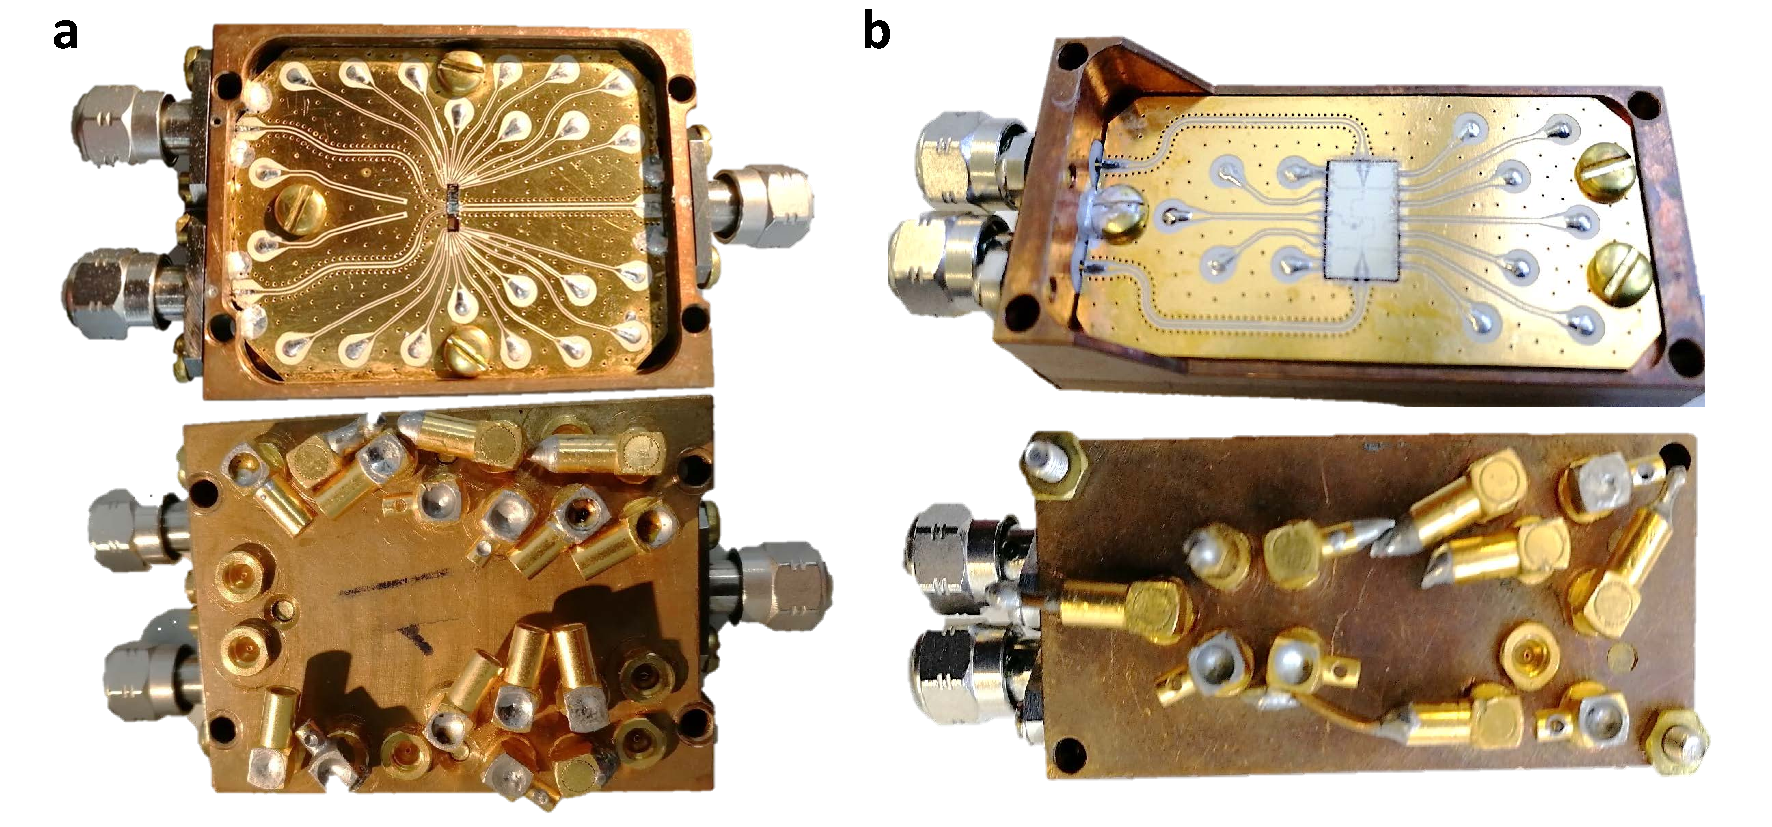
\includegraphics[width=\textwidth]{polished/PCB.pdf}
	\caption[PCB]{\textbf{a}. a }
	\label{fig:pcb}
\end{figure}

To connect our samples to electronics we use a printed circuit board (PCB) inside a copper enclosure as shown in figure \ref{fig:pcb}. These PCBs have been carefully designed with impedance matched lines for all high frequency ports and spare ports to accommodate for design changes. The dipole PCB (Fig. \ref{fig:pcb}a) holds two pixels which makes chip handling slightly easier as the pixel size is only $1.4\times1.4\,$mm. It features two high frequency SMA
and one SK line and 22 MMCX lines. The CPWR PCB (Fig. \ref{fig:pcb}b) holds one pixel and has two SMA and 12 MMCX lines. 

The device is mounted in the PCB opening with PMMA and subsequently connected to the PCB lines with an aluminium wedge wire bonder. Fast frequency lines are bonded as matched as possible by using many short bonds. The CWPR requires many additional bonds (from PCB ground to sample ground and across the different ground sections on the sample) to properly secure the ground plane is equal over the entire chip. During the bonding process all lines remain grounded to avoid electrostatic discharge (ESD) damage. 

\section{Experimental setup} \label{sec:setup}

Our experiments are performed at low temperatures ($\sim 11\,$mK) to prevent spurious thermal excitation as much as possible. Cryogen-free dilution refrigerators (BlueFors LD400 and ??) can achieve these temperatures by  exploiting the enthalpy of mixing of $^4$He and $^3$He. The coldest part of the fridge is where the gases mix and is fittingly called the mixing chamber. There we attach our sample enclosures with our qubits on a cold finger. The fridge is outfitted with a superconducting magnet. The qubit sits in the center of this magnet and thus experiences a homogeneous magnetic field of up to 5 T.

In this thesis three different types of qubits are discussed: the standard electron and nuclear qubit (see chapter \ref{Chapter1} and \ref{Chapter7}), the flip-flop qubit implemented with direct dipole-dipole coupling and resonator coupling (see chapter \ref{Chapter2, Chapter3, Chapter4, Chapter6}). These different qubits have different demands on the measurement setup which will be explained in the following sections. 

\subsection{Electron qubit} \label{sec:setup_en}

\subsubsection{Cables and filtering}

\begin{figure}
	\centering
	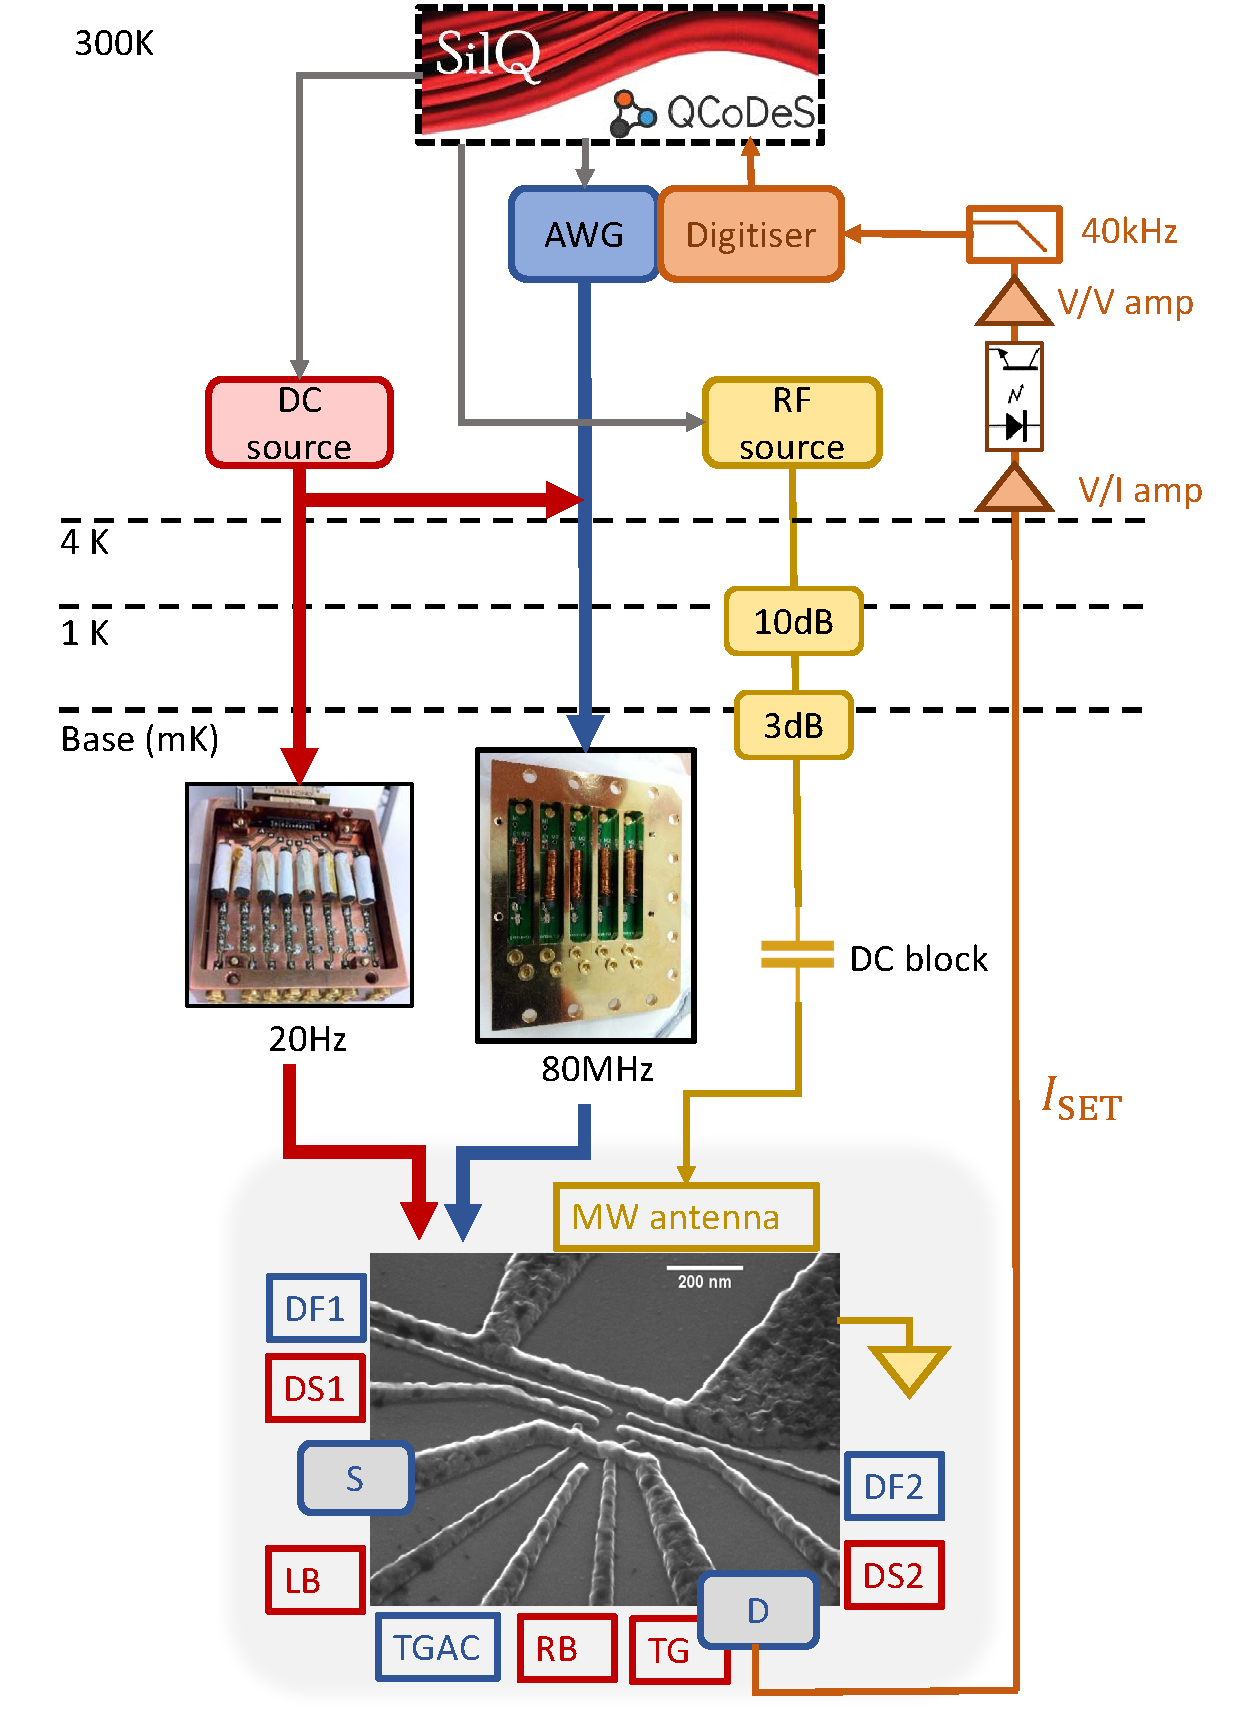
\includegraphics[width=\textwidth]{polished/wiring_queenie.pdf}
	\caption[Electron qubit setup]{\textbf{Electron qubit setup}. Detailed schematics of the experimental setup for the electron qubit.  }
	\label{fig:queenie_setup}
\end{figure}

The qubit has three distinct types of connections to the room temperature world outside of the dilution refridgerator: DC, AC and high frequency ($>80\,$MHz). Each type of connections aims to allow a sufficient amount of power down to the qubit while simultaneously minimizing any thermal noise. Any electrical line emits thermal white noise, called Johnson-Nyquist noise \cite{Johnson, Nyquist} with a power spectral density of $v_n^2=4k_BTR$, where $T$ is the temperature and $R$ the resistance of said line. This noise can be reduced either by attenuation or filtering. We choose our approach according to the line type. 
Figure \ref{fig:queenie_setup} shows the schematic of the line attenuation,  filtering and instrument control used for the electron and nuclear qubit. 

The DC lines require a fixed voltage bias and consist out of the left (LB) and right (RB) SET barrier, the SET top gate (TG), and two donor gates (DS1, DS2). To minimize the Johnson-Nyquist noise as much as possible we filter these lines with a handmade filter box that acts as a low pass filter and attenuates any signal above 20 Hz. It consists out of two passive first-order RC filters in series, with thin-film nichrome resistors of $20\,k\Omega$ and $470\,$nF and $1\,$pF ceramic capacitors, resulting in cut-off frequencies of $20\,$Hz and $8\,$MHz respectively. The lines running from room temperature to the filter box are copper-nickel twisted-pair wires that are thermalized at every temperature stage. 
The AC lines - two more donor gates (DF1, DF2), source (S), drain (D) and the plunger gate (TGAC) - require a fixed voltage bias, but also slow pulsing. Thus we use coppernickel semi-rigid (EZ86) coaxial lines and a filter box with a cut-off frequency of $80\,$MHz instead, consisting of seventh-order integrated LC filters (Mini-Circuits LFCN-80). 
In addition to the passive filters, both filter boxes contain an anti-inductive wound coil with an Eccosorb core in series to reduce high-frequency noise.  Connections from the filter boxes to the enclose are made with MMCX cables. 

The high frequency line needs to transmit pulses of up to $40\,$GHz, thus cannot be filtered. Consequently we use attenuators at different temperature stages to create a good thermal contact between the coaxial signal line of the semi-rigid stainless steel (EZ86) cable and the ground shield which in turn is thermalized to the fridge using copper anchors. These size of the attenuators depends on the required power at the sample and the cooling power at the respective temperature stage. 
We place 10dB of attenuation at 1K and 3dB at mK, which results in a noise temperature of 2K\footnote{300K room temperature noise gets reduced by a factor 10 (10dB) at 4K, leading to 30K additional noise. 34K thermal noise at 4K gets reduced by a factor 2 (3dB) at mK, leading to thermal noise of temperature 17K at the sample}. 
Additionally we add a DC block at mK to remove any DC noise. 

\subsubsection{Instrument control}
All instruments are controlled with our home-built measurement software SilQ \cite{SilQ} which is a python environment built on top of the shared quantum measurement package QCoDes \cite{QCodes}. DC voltages are applied with PXI voltage source card in the measurement computer, directly controlled with SilQ. A TTL pulse generator (SpinCore PulseBlasterESR-PRO) controlled by SilQ is used to trigger all pulses to ensure proper pulse alignment. AC voltages are also supplied by the PXI, however for TGAC, DF1 and DF2 the DC voltage is combined by a resistive combiner with a pulse from the Lecroy ArbStudio arbitrary waveform generator (AWG). ESR pulses are generated by the Agilent E8267D Vector Source. 
The measurement signal of the device consists of the SET current, usually of magnitude of $I\sim 1\,$nA. We amplify the current using a FEMTO DLPCA-200 trans-impedance amplifier set at $10^7\,$V/A. Afterwards the voltage is further amplified by a SIM910 voltage amplifier with a gain of 10 V/V, which also acts as an opto-isolator. This prevents any large ground loop through the fridge. Finally the signal is filtered by a SIM965 analog filter module set to a low-pass fourth order Bessel filter with a cut-off frequency of 40 kHz before it is acquired with the a Keysight Sygnadyne. SilQ controls the data acquisition and transmission from the Sygnadyne temporary storage to the data hard drive.


\subsection{Flip-flop qubit dipole-coupled} \label{sec:setup_dd}

\begin{figure}
	\centering
	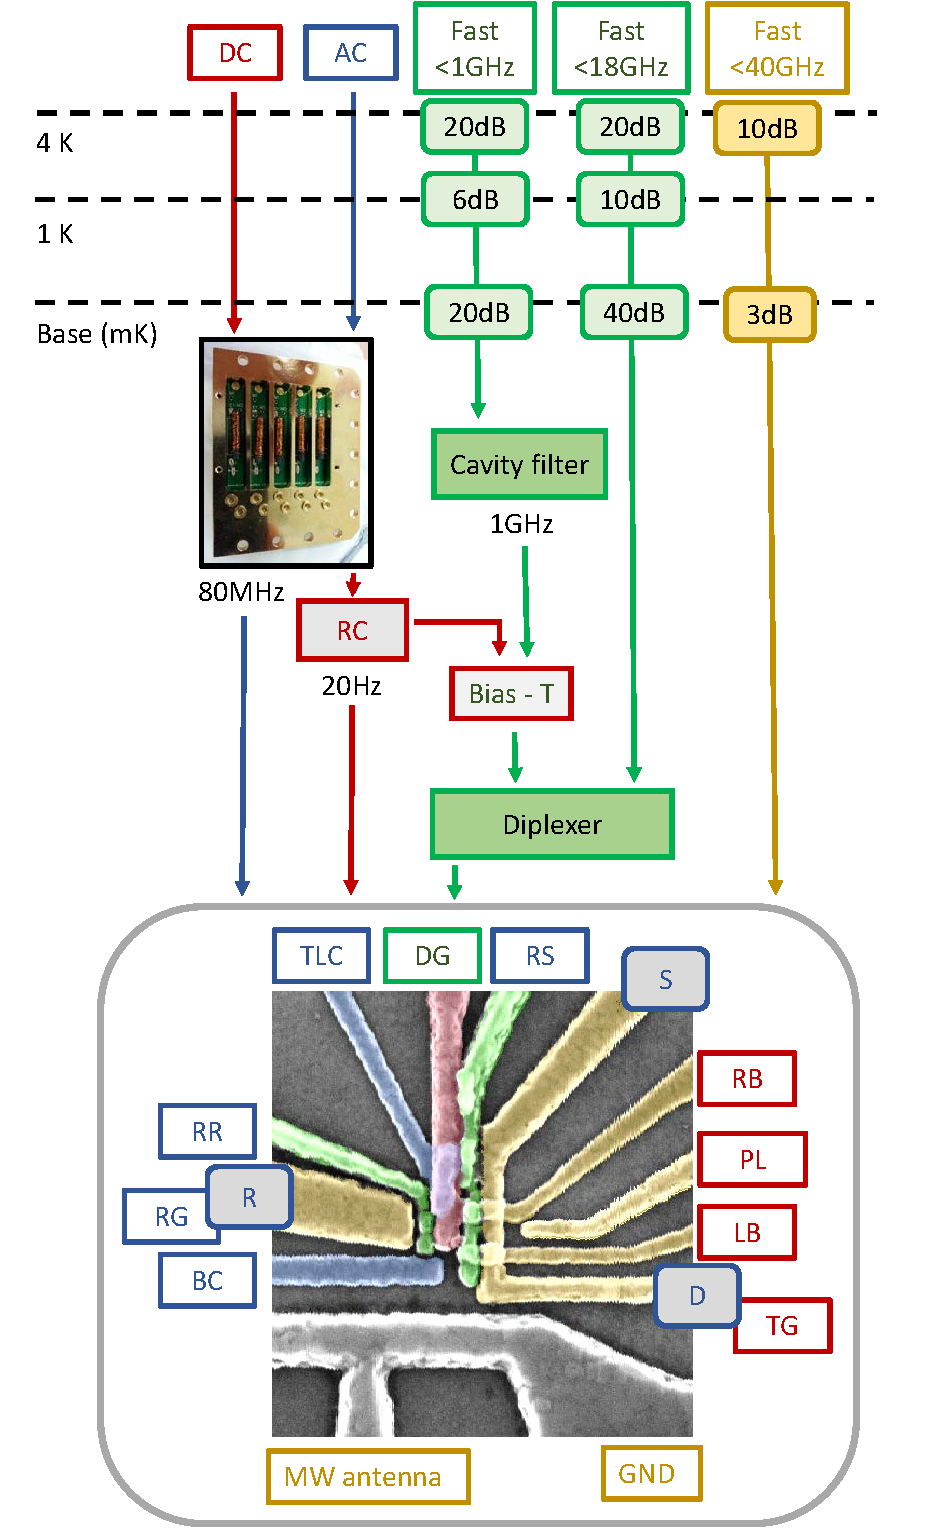
\includegraphics[width=1\textwidth]{polished/wiring_ff.pdf}
	\caption[Flip-flop qubit setup]{\textbf{Flip-flop qubit setup}. Detailed schematics of the experimental setup for the dipole-coupled flip-flop qubit.  }
	\label{fig:dd_setup}
\end{figure}

The setup for the dipole coupled flip-flop qubit (Fig. \ref{fig:dd_setup}) is very similar to the standard electron qubit setup. The qubit has 5 DC lines (RB, LB, TG,  TLC and BC), 7 AC lines (S, D, PL, RS, RR, R and RG) and the high-frequency microwave line. All these lines are wired and operated in the same fashion as for the electron qubit as is the SET readout. The distinct difference to that standard setup is that the donor gate (DG) requires both fast pulsing (GHz) as well as a DC voltage and AC pulsing. To combine these three different frequency lines we use a home-built bias-T and a diplexer XX. 

\begin{figure}
	\centering
	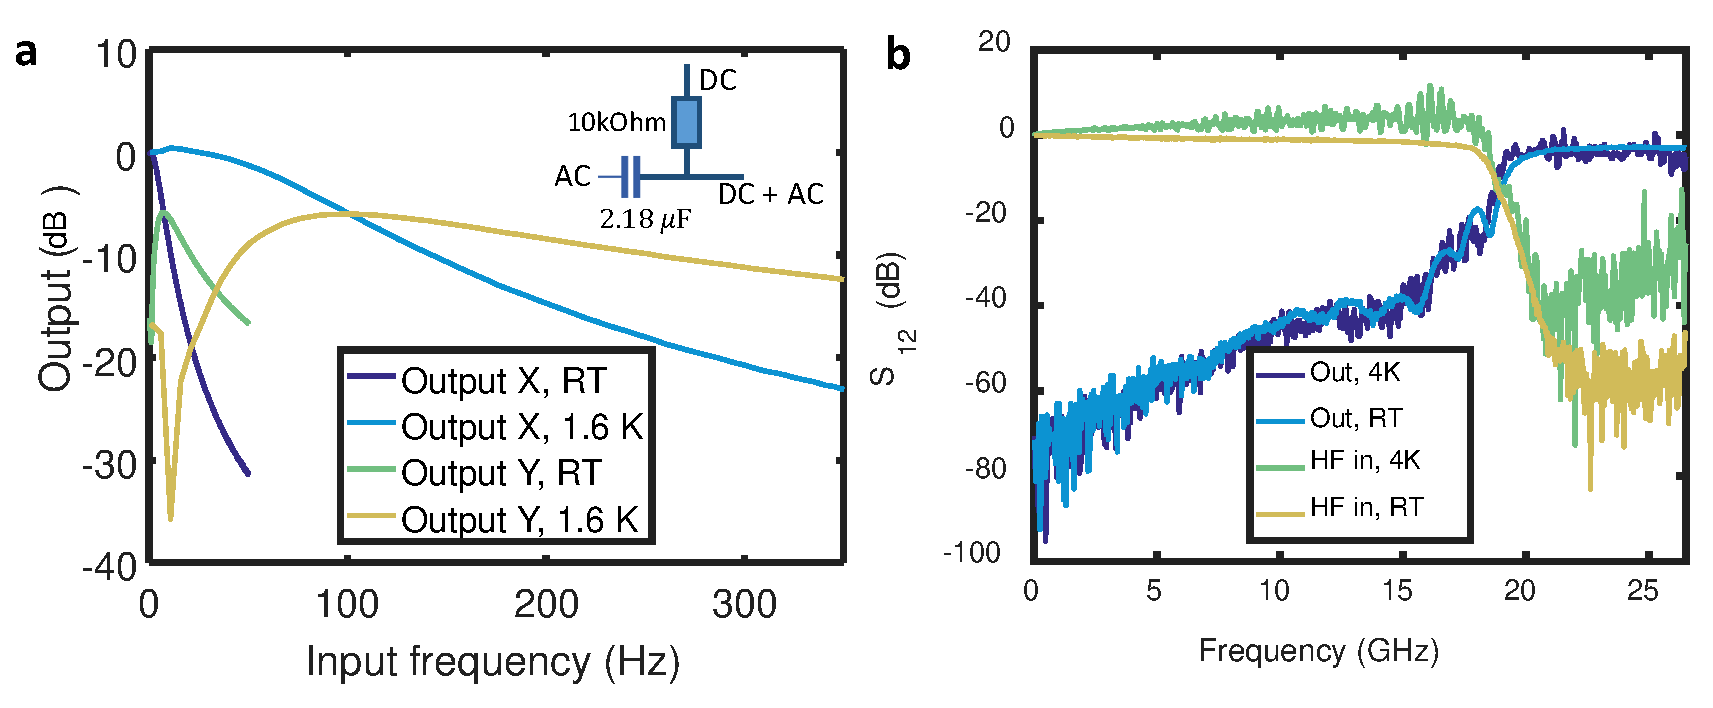
\includegraphics[width=\textwidth]{polished/ff_filtering.pdf}
	\caption[Bias-T and diplexer transmission measurements]{\textbf{Bias-T and diplexer transmission measurements. a} Bias-T transmission from AC to combined port (schematic in top corner) for in-phase(X) and out-of-phase (Y) at 1.6K and room temperature using a lock-in amplifier. The -3dB point shifts from 5Hz at room temperature to 70Hz at 1.6K. \textbf{b} Transmission of the diplexer for input high-frequency (HF) port and the output port at 4K and room temperature using a vector network analyser (VNA). The cut-off frequency is at 18GHz. }
	\label{fig:biast_diplexer}
\end{figure}

The bias-T is comprised of a 10kOhm resistor and a $2.18\,\mu$F ceramic capacitor (see inset figure \ref{fig:biast_diplexer}a) resulting in a cut-off frequency of 5Hz at room temperature which shifts to 70Hz at 1.6K, as measured in figure \ref{fig:biast_diplexer}a. We use this to combine the DC bias from the PXI modules, filtered by the 20Hz filter box, with an attenuated AC pulse from the AWG of up to 1GHz. We choose attenuators of 20dB at 4K, 10dB at 1K and 10dB at mK, giving a noise temperature of 170mK at base
 \footnote{
 %300K room temperature noise gets reduced by a factor 100 (20dB) at 4K, leading to 3K additional noise. 7K thermal noise at 4K gets reduced by a factor 10 (10dB) at 1K, leading to 1.7K additional noise at mK. 1.7K thermal noise at mK gets reduced by a factor 10, leading to a noise temperature of 170mK at the sample. 
 Assuming an applied voltage of 5mV at the sample with a $50\,\Omega$ impedance we create 500nW power dissipation at sample and $5\,\mu$W at mK which can be handled by our dilution refrigerator.}.  

The diplexer passively combines high-frequency and low-frequency pulses by frequency-domain multiplexing with a cut-off at 18GHz, as measured in figure \ref{fig:biast_diplexer}b. We connect the low-frequency port to the output of the bias-T and the high-frequency port to a microwave source with attenuators of 20dB at 4K, 10dB at 1K and 40dB at mK, resulting in a noise temperature of 15mK at base. %\footnote{300K room temperature noise gets reduced by a factor 100 (20dB) at 4K, leading to 3K additional noise. 7K thermal noise at 4K gets reduced by a factor 10 (10dB) at 1K, leading to 0.7K additional noise at mK. 1.7K thermal noise at mK gets reduced by a factor 10 000, leading to a noise temperature of 12mK at the sample. Assuming an applied power of 1pW \cite{Tosi2017} at the sample we create 10nW power dissipation at mK.} 


\subsection{Resonator qubit} \label{sec:setup_res}

\begin{figure}
	\centering
	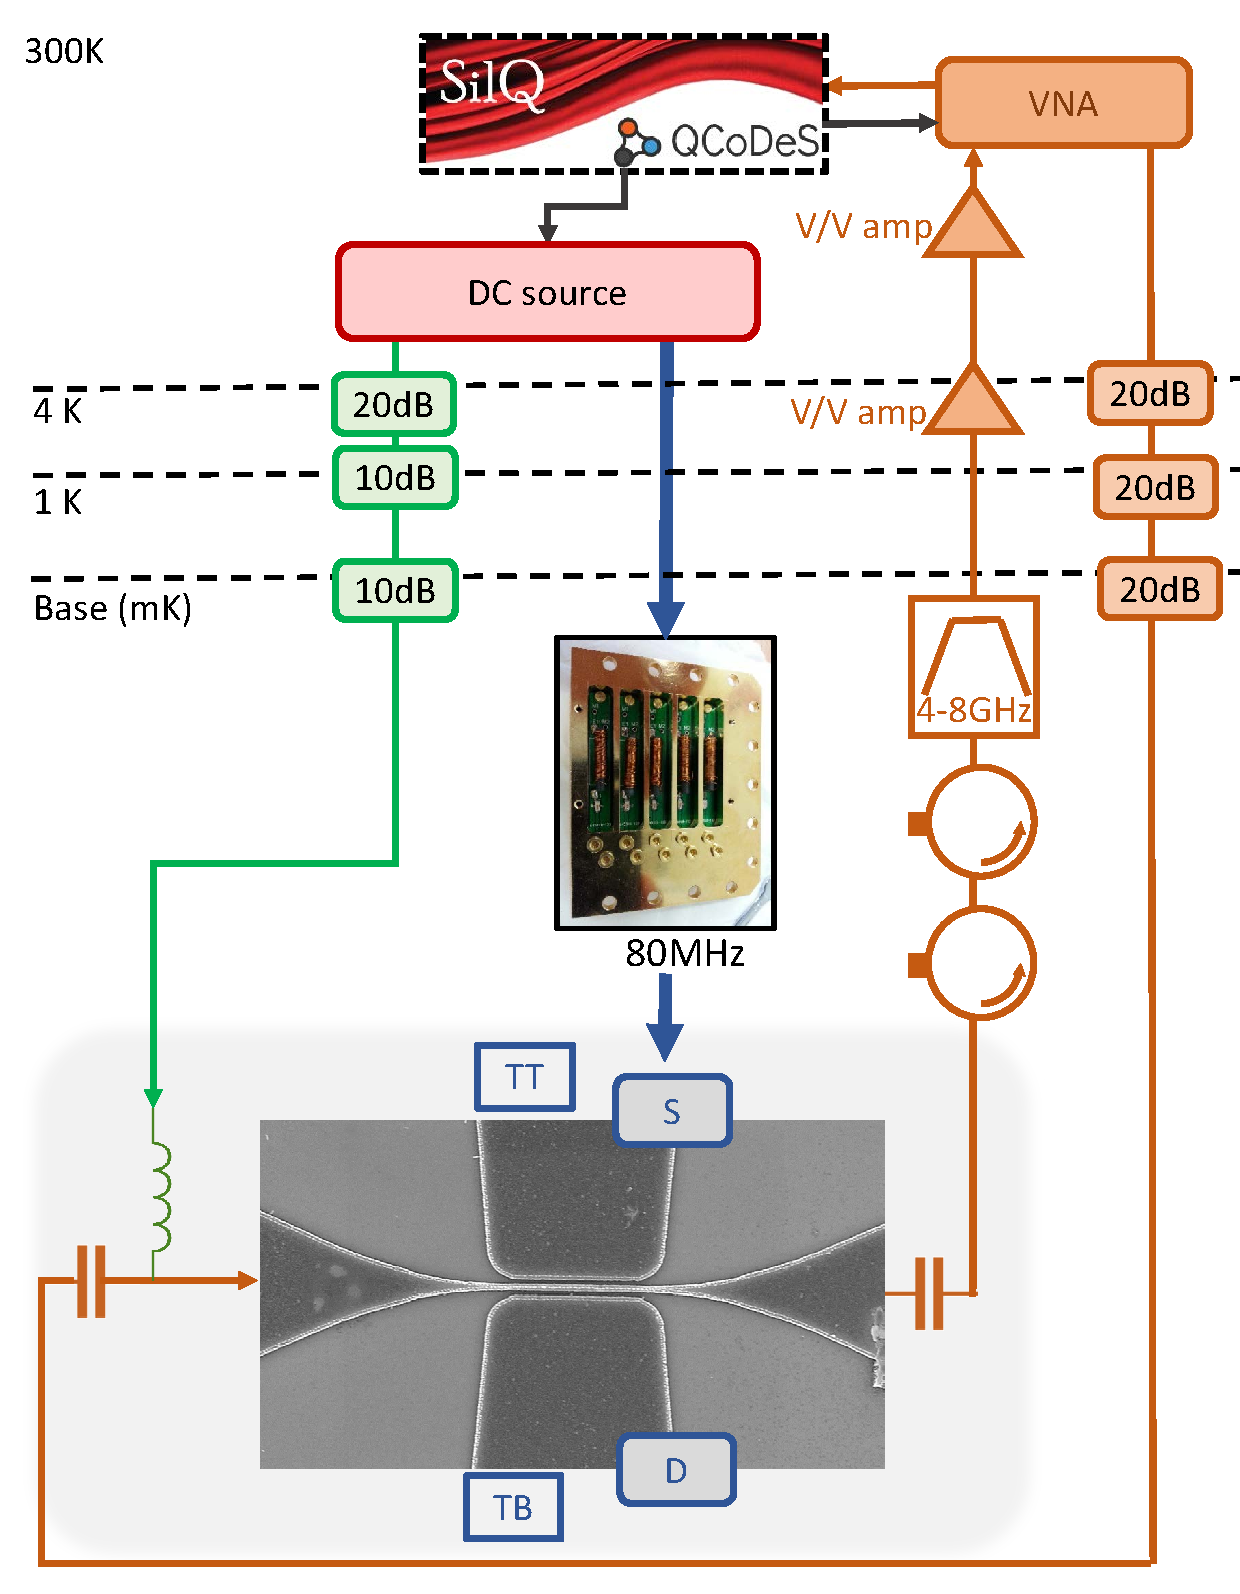
\includegraphics[width=1\textwidth]{polished/wiring_CPWR2.pdf}
	\caption[Flip-flop resonator qubit setup]{\textbf{Flip-flop resonator qubit setup}. Detailed schematics of the experimental setup for the flip-flop qubit coupled to a superconducting resonator.  }
	\label{fig:resonator_setup}
\end{figure}

When coupling our flip-flop qubit to a superconducting resonator, the setup changes significantly from our traditional electron qubit setup. In the simple resonator design the four gates (TT, TB, S, D) are connected via coppernickel semi-rigid (EZ86) coaxial lines to the 80MHz filter box and then at room temperature to the Stanford Research Systems (SRS) SIM928 Isolated Voltage Source modules in a SIM900 mainframe. These lines are thermalized at every temperature stage. 
The central conductor is biased through an on-chip inductor by the SIM module with attenuation of 20dB at 4K, 10dB at 1K and 10dB at mK, same as for the AC line of the dipole-coupled flip-flop qubit donor gate. 

Readout is performed through the resonator. We operate in transmission mode. The input signal is generated by the VNA and attenuated by 20dB at each temperature stage (noise temperature of 120mK .
%\footnote{300K room temperature noise gets reduced by a factor 100 (20dB) at 4K, leading to 3K additional noise. 7K thermal noise at 4K gets reduced by a factor 100 (20dB) again at 1K, leading to 70mK additional noise at 1.K. 1.07K thermal noise at 1K gets reduced by a factor 100, leading to a noise temperature of 120mK at the sample.}). 
The output signal is routed through two isolators to reduce any thermal noise coming down the line and a 4-8 GHz bandpass filter to reduce any noise before amplification. The signal then passes a cryogenic amplifier with dB gain and a room temperature amplifier with dB gain before entering the VNA. SilQ controls the SIM modules and the VNA. 

\subsubsection{Advanced resonator design}

\begin{figure}
	\centering
	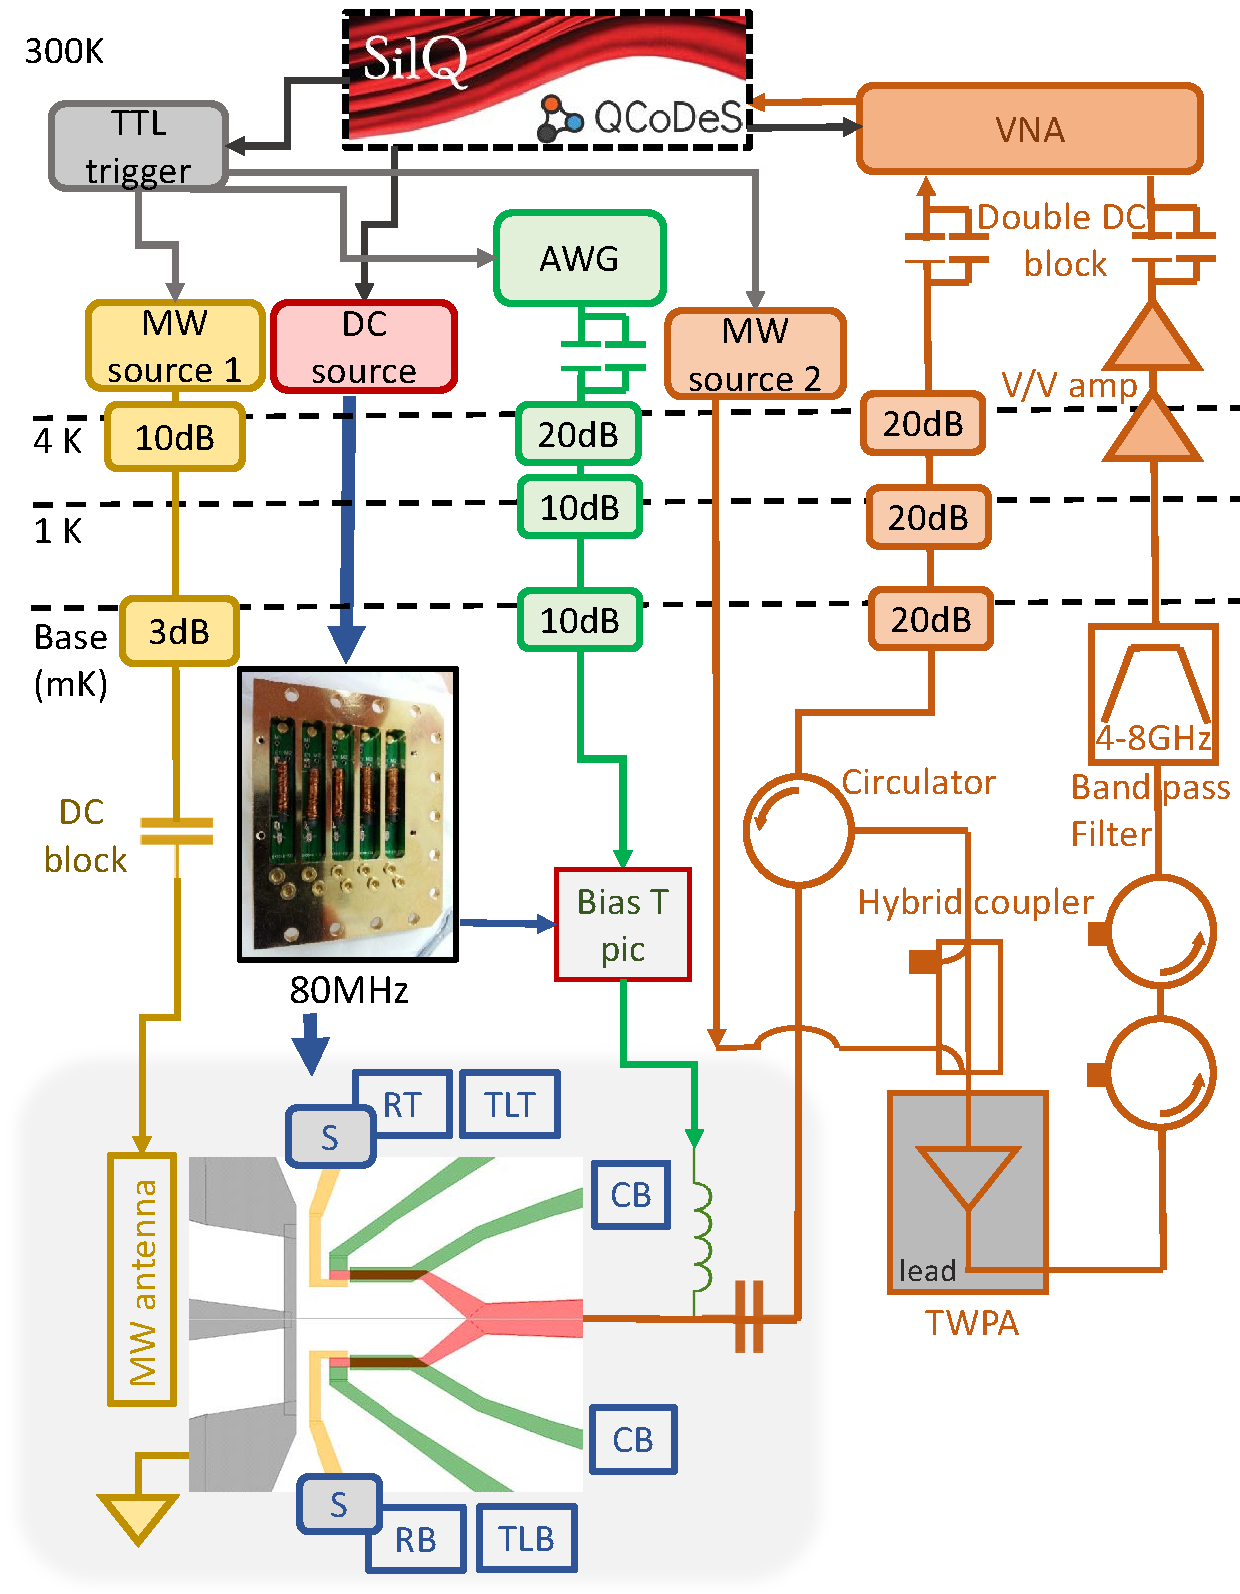
\includegraphics[width=1\textwidth]{polished/wiring_CPWR_VS.pdf}
	\caption[Advanced flip-flop resonator qubit setup]{\textbf{Advanced flip-flop resonator qubit setup}. Detailed schematics of the experimental setup for the flip-flop qubit coupled to a superconducting resonator with the advanced design.  }
	\label{fig:resonator_setup_new}
\end{figure}

The setup for the advanced resonator design is more complex as we now not only have several additional gates and a microwave antenna but also are operating the resonator in reflection. It is basically a hybrid between the simple resonator design and the dipole design with some additional components for good reflective resonator operation.

The microwave antenna and the AC gates (S, RT, TLT and CB) are connected as for the dipole-coupled qubit in section \ref{sec:setup_dd}, with difference that each gate has its own on-chip inductor to reduce coupling into the resonator.  
The central conductor is biased through the on-chip inductor as for the simple resonator design. However, we prefer to use a bias-T as for the dipole design to better filter the line. 

The resonator is connected on one port only where the signal is send in, reflected and then measured. 
The signal is generated by the VNA, attenuated by 20dB on each temperature stage, passes through a circulator and reaches the resonator. Then the signal is reflected, travels up the same line, enters the circulator where it is separated from the input signal. It is then fed into a hybrid coupler where the signal is combined with a pump tone from a second microwave source of a frequency and power calibrated to the signal. This tone is required at the next stage, the Josephson travelling-wave parametric amplifier (TWPA), which amplifies the signal up to 20dB over a 3GHz bandwidth \cite{Macklin2015}. Following is the same readout setup as for the simple design. We add double-DC blocks on all high-frequency lines to reduce DC current noise. 




